\documentclass{article}
\usepackage[utf8]{inputenc}
\usepackage[T1]{fontenc}
\usepackage{amsmath}
\usepackage{graphicx}
\usepackage{amssymb}
\usepackage{float}
\usepackage{tikz}
\usepackage{pgfplots}
\usepackage[letterpaper, margin=1in]{geometry}
\usepackage{hyperref}
\hypersetup{
	colorlinks=true,
	linkcolor=blue,
	citecolor=blue,
	filecolor=blue,      
	urlcolor=blue,
	pdftitle={Concealed Bike Anti-Theft Device},
	pdfpagemode=FullScreen,
}


\begin{document}
	
	\begin{titlepage}
		\title{Concealed Bike Anti-Theft Device: Requirements \& Verification Tables}
		\author{Elizabeth Atkinson (eatkinso)\\ Srinidhi Raman (nidhim2) \\ Alex Wen (acwen2) }
	\end{titlepage}
	
	
	
	\maketitle{}
	
\section{High-Level Requirements}

\begin{enumerate}
	\item If a user tries to remove the bike from a stationary location without the RFID tag, the alarm will sound. 
	
	\item The device receives GPS data \textit{at least} once per minute, and records its own position over time.  
	
	\item The device transmits its GPS location data and additional data over LoRa to be received by a base station. 
	
\end{enumerate}

\section{Requirements and Verification}

\subsection{Control Subsystem Requirements \& Verification}

\begin{figure}[H]
	\begin{centering}
		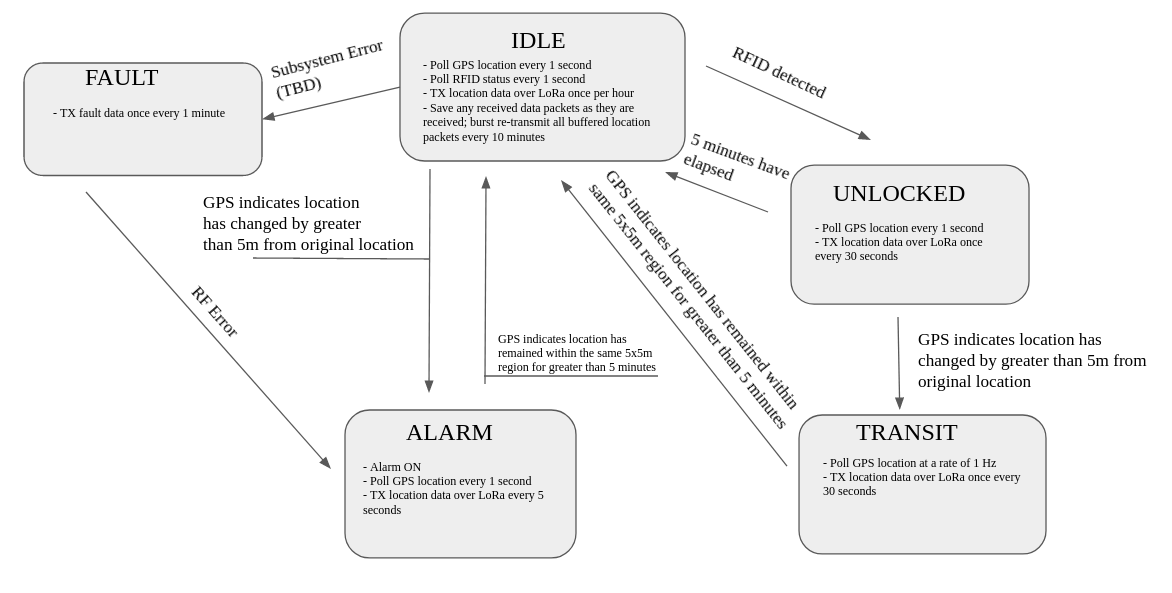
\includegraphics[width=\textwidth]{state.png}
		\caption{Control System State Machine}\label{state}
	\end{centering}
\end{figure}

\begin{figure}[H]
	\begin{center}
		\begin{tabular}{|p{0.3 \linewidth}|p{0.6 \linewidth}|}
			\hline
			Requirement & Verification  \\
			\hline
			\begin{enumerate}
				\item  The microcontroller implements a state-based control system with power-saving measures in the idle/safe states.  
			\end{enumerate} &
			\begin{enumerate}
				\item Flash the firmware to the device. 
				\item Monitor the state transitions during device operation. 
			\end{enumerate}  \\
			\hline
			\begin{enumerate}
				\item The microcontroller packetizes data to be sent over LoRa at the update rate specified by the state diagram in figure \ref{state}.
			\end{enumerate} & \begin{enumerate}
				\item Flash test firmware that cycles through each of the states. 
				\item Verify that the TX update rate is greater than once per hour in the IDLE, UNLOCK, and TRANSIT states. 
			\end{enumerate} \\
			\hline 
		\end{tabular}
	\end{center}
	\caption{Microcontroller R\&V Table.}
\end{figure}


\subsection{LoRa Subsystem Requirements and Verification:}

\begin{figure}[H]
	\begin{center}
		\begin{tabular}{|p{0.3 \linewidth}|p{0.6 \linewidth}|}
			\hline
			Requirement & Verification  \\
			\hline
			\begin{enumerate}
				\item The LoRa subsystem matching network and antenna have a VSWR of less than 10 at the RF output of the STM32WL55CC. 
			\end{enumerate}  & \begin{enumerate} 
				\item Populate the RF matching network before populating the microcontroller.
				\item Calibrate the VNA from 800-1200 MHz with PCB TRL standards. 
				\item Terminate the SMA output of the PCB with a 50 ohm load.
				\item Measure the input impedance looking into the RF matching network at the RF output of the STM32WL55CC.
				\item Calculate the VSWR from the measured input impedance and the specified PA output impedance in the STM32 datasheet. 
			\end{enumerate}
			\\
			\hline
			\begin{enumerate}
				\item The antenna is hidden in a common bike component such as a reflector so that it is not visibly obvious. 
			\end{enumerate}  & \begin{enumerate}
				\item Objective visual verification. 
				\item Ask other senior design students.
			\end{enumerate} \\
			\hline
		\end{tabular}
	\end{center}
	\caption{LoRa Subsystem R\&V Table.}
\end{figure}

\textit{\textbf{Note:}} The LoRa Subsystem does not function as desired. When the radio is set to the TX state, there is no RF output (measured with a spectrum analyzer). Since identical code \textit{does} successfully transmit CW on the Nucleo development board, this is likely due to a hardware error. We have several possible explanations and future solutions for this failure: 

\begin{enumerate}
	\item \textbf{Oscillator:} Our PCB had an error in the oscillator footprint, so we instead soldered a through-hole crystal oscillator to the pads. However, this introduces significant parasitic capacitance and/or inductances compared to the original SMD oscillator. This could have caused internal errors in the sensitive PLL for the RF circuitry in the STM32WLCC. This hypothesis is supported by the fact that during testing, querying the radio error status sometimes resulted in PLL Lock error. We were unable to fix this error during the course because we did not have the time or resources to order a new PCB when we discovered the error. \textbf{Solution}: Order a new board with a properly routed SMD oscillator. 
	\item \textbf{Matching Network:} During the debugging process, we depopulated the RF switch and replaced it with a small piece of wire. Since the length of the wire (approx. 4mm) was much smaller than the wavelength at 915 MHz, we assumed this would slightly degrade the VSWR but probably not cause major issues. It is possible that this change actually significantly effected the VSWR and caused the internal PA output of the radio to be destroyed. Additionally, we did not verify the self-resonant frequency of the capacitors and inductors used in the matching network due to time constraints during the part ordering process. This could also have contributed to degrading the VSWR and damaging the internal PA of the STM32WLCC. \textbf{Solution:} Verify that the capacitors and inductors are appropriate for the matching network, and verify the matching network with a VNA before use. 
\end{enumerate}

Additionally, we were also unable to verify Requirement 1 due to the fact that the lab does not have a VNA available. 


\subsection{GPS Subsystem Requirements and Verification:}

\begin{figure}[H]
	\begin{center}
		\begin{tabular}{|p{0.3 \linewidth}|p{0.6 \linewidth}|}
			\hline
			Requirement & Verification  \\
			\hline
			\begin{enumerate}
				\item   The GPS module can communicate with the microcontroller at a update rate of greater than 1 Hz.  
			\end{enumerate} &
			\begin{enumerate}
				\item  Flash a test program to the microcontroller that continuously polls the GPS module.
				\item Verify that the GPS module transfers GPS data at an update rate of greater than 1 Hz.
			\end{enumerate}  \\
			\hline 
		\end{tabular}
	\end{center}
	\caption{GPS R\&V Table.}
\end{figure}

\subsection{RFID Subsystem Requirements \& Verification:}


\begin{figure}[H]
	\begin{center}
		\begin{tabular}{|p{0.3 \linewidth}|p{0.6 \linewidth}|}
			\hline
			Requirement & Verification  \\
			\hline
			\begin{enumerate}
				\item The RFID detector will detect the user’s RFID tag within 10 seconds. 
			\end{enumerate}  & \begin{enumerate} 
				\item Place the RFID tag within 10 cm of the RFID receiver. 
				\item Monitor the RFID output data to verify it has detected the RFID card within 10 seconds.
			\end{enumerate}
			\\
			\hline
			\begin{enumerate}
				\item The RFID subsystem will provide a visual indication that the RFID tag has been detected within 1 second of detecting the RFID tag. 
			\end{enumerate}  & \begin{enumerate}
				\item Place the RFID tag within 10 cm of the RFID receiver. 
				\item Monitor the RFID reader output data and the RFID LED to verify that it turns on within 10 seconds of detecting the RFID tag. 
			\end{enumerate} \\
			\hline
			\begin{enumerate}
				\item The RFID subsystem triggers the alarm if movement occurs and the user's RFID is not detected.
			\end{enumerate}  & \begin{enumerate}
				\item Ensure that the RFID tag is out of range (> 1 m).
				\item Move the bike 5m from the original location to verify the alarm is triggered.
			\end{enumerate} \\
			\hline
			\begin{enumerate}
				\item The RFID indicator LED is concealed in an unobtrusive location on the bike.
			\end{enumerate}  & \begin{enumerate}
				\item Visual verification.
			\end{enumerate} \\
			\hline
		\end{tabular}
	\end{center}
	\caption{RFID Subsystem R\&V Table.}
\end{figure}

\subsection{Power Subsystem Requirements \& Verification:}

\begin{figure}[H]
	\begin{center}
		\begin{tabular}{|p{0.3 \linewidth}|p{0.6 \linewidth}|}
			\hline
			Requirement & Verification  \\
			\hline
			\begin{enumerate}
				\item The power system will provide 3V3 +/- 0.4 mV to all subsystems that require 3V3, and 5V to the subsystems that require 5V. 
			\end{enumerate}  & \begin{enumerate} 
				\item A multimeter will be used to ensure the voltage and current are as specified at different points on the board.
			\end{enumerate}
			\\
			\hline
			\begin{enumerate}
				\item The power system will power the device for over 24 hours. 
			\end{enumerate}  & \begin{enumerate}
				\item Connect a multimeter/oscilloscope to measure the voltage at the battery terminals. 
				\item Record data every two hours over two 12 hour periods. 
				\item The data from the device will be read to ensure that the values were reasonably constant over time.
			\end{enumerate} \\
			\hline
			\begin{enumerate}
				\item The microcontroller can fully power off the GPS and RFID subsystems when not in use by turning off the load switches. 
			\end{enumerate}  & \begin{enumerate}
				\item Flash a test program to the micrcontroller that toggles the control signals GPS\_~PWR and RFID\_~PWR. 
				\item Measure the output voltage on pin 1 of U7 and U8 to verify that the RFID and GPS subsystems are powered off. 
			\end{enumerate} \\
			\hline
		\end{tabular}
	\end{center}
	\caption{Power Subsystem R\&V Table.}
\end{figure}

\textit{\textbf{Note:}} Since the GPS requires some time to lock, we have not implemented the power-saving feature in the Demo firmware. However, we did verify in the lab that the load switches turn off power to the devices. 




\subsection{Alarm Subsystem Requirements \& Verification:}


\begin{figure}[H]
	\begin{center}
		\begin{tabular}{|p{0.3 \linewidth}|p{0.6 \linewidth}|}
			\hline
			Requirement & Verification  \\
			\hline
			\begin{enumerate}
				\item The alarm makes noise when triggered by the ALARM\_CTRL signal. 
			\end{enumerate}  & \begin{enumerate}
				\item Flash a test program to the microcontroller that toggles the ALARM\_CTRL signal.
				\item Verify that when ALARM\_CTRL=1, the alarm makes noise. 
			\end{enumerate} \\
			\hline
			\begin{enumerate}
				\item The alarm circuit draws < 1 uA of current when not making noise.
			\end{enumerate}  & \begin{enumerate}
				\item Set ALARM\_CTRL to 0 through code.
				\item Use multimeter to measure voltage and current value from the alarm.
			\end{enumerate} \\
			\hline
		\end{tabular}
	\end{center}
	\caption{Alarm Subsystem R\&V Table.}
\end{figure}

\textit{\textbf{Note:}} ALARM\_CTRL is not a signal that is 1 or 0 but instead a PWM output that is either on or off. 


\subsection{Base Station Subsystem Requirements \& Verification:}

\begin{figure}[H]
	\begin{center}
		\begin{tabular}{|p{0.3 \linewidth}|p{0.6 \linewidth}|}
			\hline
			Requirement & Verification  \\
			\hline 
			\begin{enumerate}
				\item  The receiver board will interface with the computer over USB.
			\end{enumerate}  & \begin{enumerate}
				\item Flash a test program to the base station board that sends continuous data over the I2C/USB interface.
				\item Connect the base station board to the user computer and view the data sent over USB. 
				\item Verify the received data matches the sent data. 
			\end{enumerate} \\
			\hline
			\begin{enumerate}
				\item The receiver board will receive LoRa packets from the bike-based device. 
			\end{enumerate}  & \begin{enumerate}
				\item Flash a test program to the TX (bike system) board that transmits continuous data. 
				\item Flash a test program to the RX (base station) board that listens for data and continuously sends received data to the computer over I2C (USB to the computer). 
				\item Verify the data sent from the TX board is received by the RX board.
			\end{enumerate} \\
			\hline
			\begin{enumerate}
				\item The GUI will display GPS data over the past day, week, month, or year on a map. 
			\end{enumerate}  & \begin{enumerate}
				\item Flash a test program to the TX (bike system) board that transmits data with (false) timestamps that cover a 6-month period. 
				\item Transmit the data and receive it with the base station board. 
				\item Using the GUI, plot the data and verify the output plots match the data sent by the TX board. 
			\end{enumerate} \\
			\hline
			\begin{enumerate}
				\item The GUI will allow the user to view plots of the average speed and distance traveled.
			\end{enumerate}  & \begin{enumerate}
				\item Flash a test program to the TX (bike system) board that transmits data with (false) timestamps that cover a 6-month period. 
				\item Transmit the data and receive it with the base station board. 
				\item Using the GUI, plot the average speed and distance traveled and verify that it matches the data transmitted by the bike system board. 
			\end{enumerate} \\
			\hline
			
		\end{tabular}
	\end{center}
	\caption{Base Station Subsystem R\&V Table.}
\end{figure}


\end{document}
